\documentclass[../../main.tex]{subfiles}
\begin{document}

\subsection*{4.5}
Cinque fogli metallici sferici di spessore trascurabile tutti concentrici aventi raggio pari a 1, 2, 3, 4, 5 cm sono collegati con sottili fili conduttori come in figura.
\\Il sistema è inizialmente scarico. Una carica $q=10^{-10}\ C$ è disposta sulla superfice sferica e l'energia elettrostatica $U_e$ dell'intero sistema.
\\Determinare inoltre come variano il campo elettrostatico e l'energia elettrostatica quando: la sfera 1 è posta in contatto con la 2, la 3 è posta in contatto con la 4, la 5 con la terra.
\\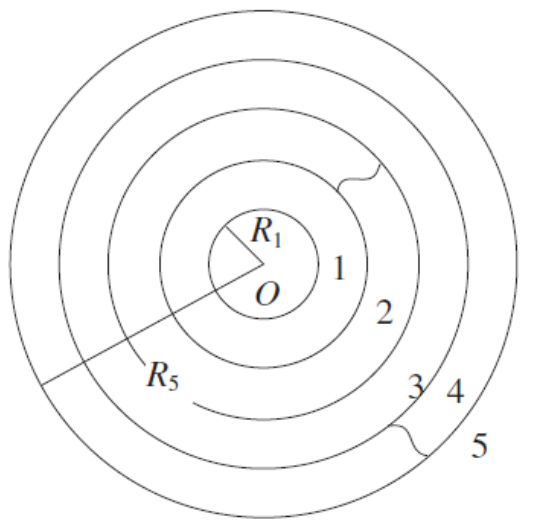
\includegraphics[scale=0.3]{e_4_5.png}
\subsubsection*{Formule utilizzate}
\subsubsection*{Soluzione punto a}
Detta $q = q_1$ la carica sulla sfera interna per induzione completa
\\$q_2 = -q$   $q_4 = -q$   $q_3 = +q$   $q_5 = +q$
\\Per calcolare il campo elettrico sfrutto la legge di Gauss e la simmetria sferica
\\$\Phi(E) = E* 4\pi r^2=\frac{Q_int}{\epsilon_0}$
\\Chiamando I la regione di spazio $r < 1\ cm$, II quella con $1\ cm < r<2\ cm$ e così via, si ha che.
\\$E_I = E_{III} = E_V = 0$
\\$E_{II} = E_{IV} = E_{VI} = \frac{q}{4\pi\epsilon_0r^2}$
\\L'energia elettrostatica $U_e$ del sistema si può calcolare dalla sua definizione.
\\$U_e = \int_\tau dU_e = \int_\tau\frac{1}{2}\epsilon_0E^2d\tau$
\\L'integrale si può spezzare sulle varie ragioni di cui si è già calcolato
\\$U_e = \int_\tau dU_e = \frac{1}{2}\epsilon_0\int_r^R \frac{q^2}{16\pi^2\epsilon_0^2r^4}4\pi r^2dr = \frac{q^2}{8\pi\epsilon_0}\left[\frac{1}{r}-\frac{1}{R}\right]$
\\$U_e = U_e^{II} + U_e^{IV} + U_e^{VI} = \frac{q^2}{8\pi\epsilon_0}\left[\frac{1}{R_1}-\frac{1}{R_2}+\frac{1}{R_3}-\frac{1}{R_4}+\frac{1}{R_5}\right]$
\\Collegando oltre alla sffera 2 e 3, 4 e 5, già connesse, ache la 1 alla 2 si ha:
\\$E_I=E_{II} = E_{III}= E_V = 0$
\\$E_{IV} = E_{VI} = \frac{q}{4\pi\epsilon_0 r^2}$
\\Dunque calcolando l'energia, rispetto alla situazione di partenza, si azzera il contributo della regione II.
\\$\Delta U_e = \frac{q^2}{8\pi\epsilon_0}\left[\frac{1}{R_2}-\frac{1}{R_1}\right] = -2.2 * 10^{-9}\ J$
\\Invece collegando al sfera 2 e 3, 4 e 5 già connesse, anche al 5 a terra si ha che:
\\$E_I = E_{III} = E_V = E_{VI} = 0$
\\$E_{II} = E_{IV} = \frac{q}{4\pi\epsilon_0 r^2}$
\\Dunque calcolando l'energia rispetto alla situazione di partenza, si azzera il contributo della regione VI.
\\$\Delta U_e = \frac{q^2}{8\pi\epsilon_0}\left[-\frac{1}{R_5}\right] = -0.9*10^{-9}\ J$
\subsubsection*{Soluzione punto b}
\newpage

\end{document}